\documentclass{beamer}

\usepackage[ngerman]{babel}
\usepackage{graphicx} % fuer Bilder
\usepackage{listings} % fuer Code

\usetheme{Goettingen}

\lstset{language=C++} % fuer c++ code style

\title{Prozesslenkung: Hierarchische Zustandsautomaten II}
\subtitle{Implementierung Hierarchischer Zustandsautomaten}
\author{Katja Kirstein, Anne-Lena Kowalka, Marian Triebe, Eugen Winter}
\date{\today} 

\begin{document}
\begin{frame}
\titlepage
\end{frame}

%% Themen uebersicht
\begin{frame}
 \frametitle{Themen}
 \begin{itemize}
  \item Grundlagen GoF
  \item Externe Statevariablen
  \item Entry und Exit Code
  \item History
  \item Conditions/Guards/Choice Points
  \item Timer
 \end{itemize}
\end{frame}

%% GoF fsm Beispiel (Klassendiagramm)
\begin{frame}
 \frametitle{GoF State Pattern Struktur}
 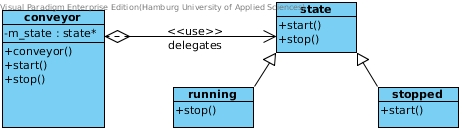
\includegraphics[scale=.6]{img/fsm_gof.jpg}
 \begin{itemize}
  \item Kontext-Klasse (conveyor)
  \item Zustands Basisklasse (state)
  \item Zust\"ande (running, stopped)
 \end{itemize}
\end{frame}

%% Grundlagen GoF
\begin{frame}
 \frametitle{Grundlagen GoF}
 Die klassiche GoF Implementierung hat einige schw\"achen
 \begin{itemize}
  \item Hoher Speicherverbrauch, da jeder State im Speicher gehalten werden muss, auch wenn diese eigentlich nicht verwendet werden
  \item Der h\"ohere Speicherverbrauch kann allerdings mit dem Placement New Operator umgangen werden
  \item Kontext muss eventuell immer mit \"ubergeben werden
 \end{itemize}
\end{frame}

%% GoF fsm Systemgrenzen
\begin{frame}
 \frametitle{Systemgrenzen}
\end{frame}

%% GoF fsm Automat
\begin{frame}
 \frametitle{Automat}
\end{frame}

%% GoF fsm States in Code I
\begin{frame}
 \frametitle{GoF States in Code I}
 \begin{itemize}
  \item Alle States erben von einer Oberstate Klasse
  \item Der Oberstate implementiert alle Events aller Zustände als leere virtuelle Funktion
  \item Der jeweilige Zustand implementiert nur seine eigenen Events, nicht relevante
  Events werden an die leeren Methoden der Basisklasse weitergereicht
 \end{itemize}
\end{frame}

%% GoF fsm States in Code (Header)
\begin{frame}[fragile]
 \frametitle{GoF States in Code (Header)}
 \begin{lstlisting}
  struct state {
    virtual ~state() { }
    virtual void start() { }
    virtual void stop() { }
  };

  struct running : public state {
    void stop();
  };

  struct stopped : public state {
    void start();
  };
 \end{lstlisting}
\end{frame}

%% GoF fsm States in Code (Implementierung/CPP)
\begin{frame}[fragile]
 \frametitle{GoF States in Code (Implementierung)}
 \begin{lstlisting}
  // transition running -> stopped
  void running::stop() {
    new (this) stopped;
    cout << "stop() / stop" << endl;
  }

  // transition stopped -> running
  void stopped::start() {
    new (this) running;
    cout << "start() / run" << endl;
  }
 \end{lstlisting}
\end{frame}

%% GoF fsm Kontext Klasse
\begin{frame}
 \frametitle{GoF Kontext Klasse}
 \begin{itemize}
  \item Sicht von au{\ss}en auf die FSM
  \item Dient als Delegator zu den States
  \item Bedient alle Eingangssignale durch Funktionen
 \end{itemize}
\end{frame}

%% GoF fsm Konext Klasse
\begin{frame}[fragile]
 \frametitle{GoF Kontext Klasse in Code}
 Header:
 \begin{lstlisting}
  struct conveyor {
    conveyor() : m_state(new stopped) { }
    ~conveyor() { delete m_state; }
    void start();
    void stop();
   private:
    state* m_state;
  };
 \end{lstlisting}
 Implementierung:
 \begin{lstlisting}
  void conveyor::start() {
    m_state->start();
  }
  void conveyor::stop() {
    m_state->stop();
  }
 \end{lstlisting}
\end{frame}

%% Schritte zum erstellen einer FSM
\begin{frame}
 \frametitle{Schritte zum erstellen einer FSM}
 \begin{enumerate}
  \item Erstellen der Systemgrenzen
  \item Erstellen einer FSM
  \item Umwandlung in Code
  \begin{itemize}
   \item Kontextklasse, Funktionsnamen als Eingangssignale
   \item Basisklasse für Zustände erstellen
   \item Zustandsklassen erben von der Basisklasse und implementieren nur die eigenen Reaktionen neu
  \end{itemize}
  \item Pr\"ufen ob Code und Systemgrenzen/Diagramm zusammenpassen
  \begin{itemize}
   \item Sind alle Eingangssignale als Funktionen zu finden?
   \item Werden alle Ausgangssignale verwendet/ausgegeben?
   \item Die Namen f\"ur Eingangssignale/Ausgangssignale sollten konsistent sein, da Fehler sonst vorprogrammiert!
  \end{itemize}
 \end{enumerate}
\end{frame}

%% Externe Statevariablen
\begin{frame}
 \frametitle{Externe Statevariablen}
\end{frame}

%% Entry/Exit Code 1
\begin{frame}
	\frametitle{Entry/Exit Code in HSM }
	\begin{itemize}
		\item das Verwenden von entry-/exit-Funktionen erfordert, dass jeder Sub- bzw. Superzustand explizit durchlaufen wird, sofern Zust\"ande nicht auf ein Signal reagieren k\"onnen
		\item der Zustandswechsel findet NICHT direkt statt
		\item exit() wird durchgef\"uhrt, wenn Signale in der Hierarchie "nach oben" weitergereicht werden 
		\item entry() wird  durchgef\"uhrt, wenn Signale in der Hierarchie "nach unten" weitergereicht werden
	\end{itemize}
\end{frame}

%% Entry/Exit Code 2
\begin{frame}
	\frametitle{Entry/Exit Code in HSM }
	\begin{itemize}
		\item Beispiel exit: State S12 erh\"alt Signal e
	\end{itemize}
	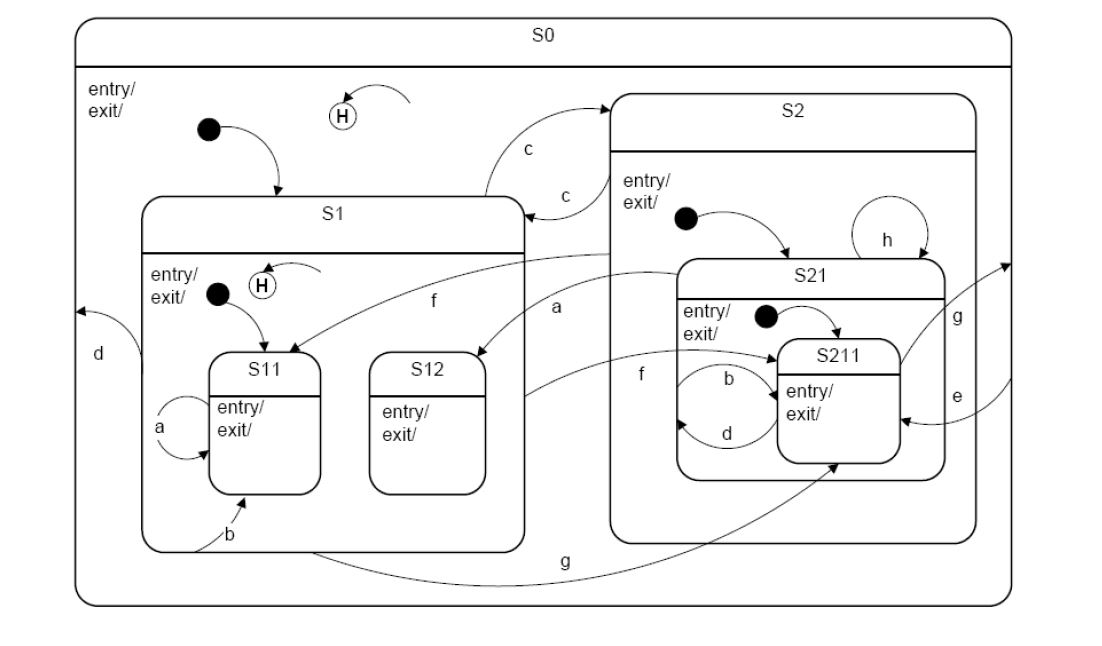
\includegraphics[scale=.3]{img/beispiel_automat}
\end{frame}

%% Exit Code 3
\begin{frame}[fragile]
	\frametitle{Entry/Exit Code in HSM }
	\begin{lstlisting}
	//State S12 erhaelt Signal e
	void StateS12::sigE() {
	exit(); 
	new (this) StateS1;
	sigE();
	}
	\end{lstlisting}
	\begin{itemize}
		\item die exit-Funktion ist in jedem Zustand definiert
		\item durch das Ueberschreiben dieses Objekts mit einem StateS1-Objekt
		zeigt der Pointer nun auf die Funktionstabelle von StateS1,
		sodass der erneute sigE-Aufruf an StateS1 delegiert wird - hieraus folgt, dass jeder Zustand eine Funktion zu jedem Ereignis haben muss
		\item wenn kein Zustand auf ein Signal reagiert, sollte der Top-Zustand z.B. eine
		failure-Methode haben, um den Fehler anzuzeigen
	\end{itemize}
\end{frame}

%% Entry Code 1
\begin{frame}
	\frametitle{Entry/Exit Code in HSM  }
	\begin{itemize}
		\item Beispiel: State S1 erh\"alt Signal b
	\end{itemize}
	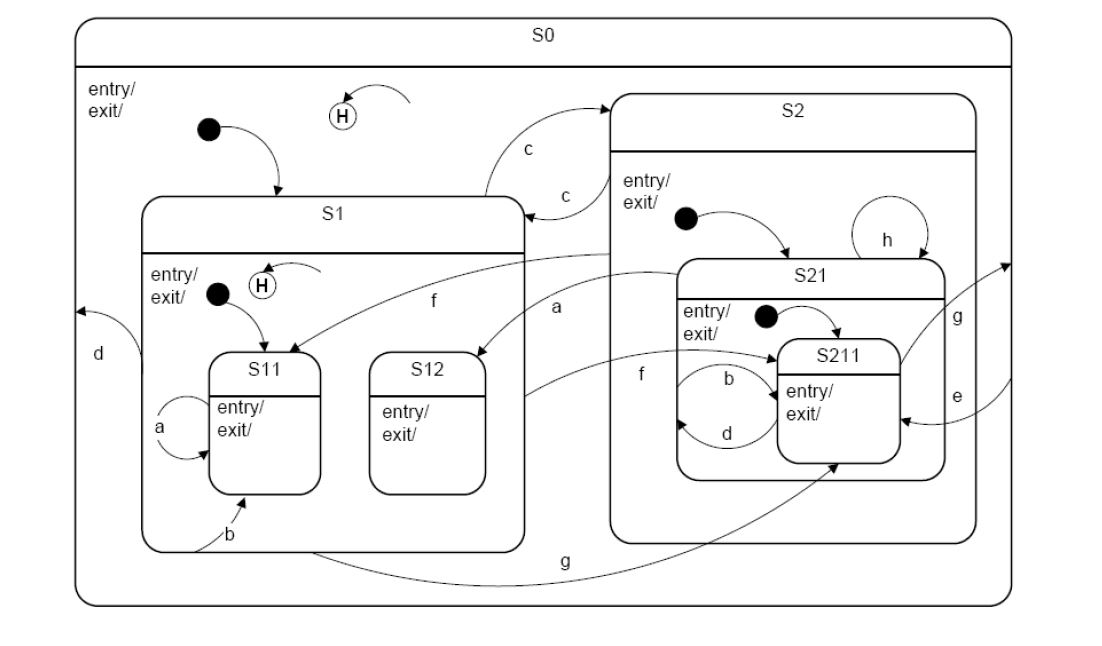
\includegraphics[scale=.3]{img/beispiel_automat}
\end{frame}

%% Entry Code 2
\begin{frame}[fragile]
	\frametitle{Entry/Exit Code in HSM }
	\begin{lstlisting}
	//State S1 erhaelt Signal b
	void StateS1::init(T* t){
	//t ist ein Pointer auf die Kontextklasse
	void* history = 
	t->getStateFromHistory(StateS1ID);
	if(history != 0){
	memcpy(this, &history, 4);
	}
	else{
	new (this) StateS11;
	entry();
	}
	init();
	}
	\end{lstlisting}
\end{frame}

%% Entry Code 3
\begin{frame}[fragile]
	\begin{itemize}
		\item die entry-Funktion ist in jedem Zustand definiert
		\item die init-Funktion definiert einen Initialzustand
		\item wenn ein Superstate sich bereits einen Substate gemerkt hat, wird dieser direkt betreten, andernfalls wird der Substate neu erzeugt
		\item init() wird in jedem Fall aufgerufen, d.h. zustandsspezifische Einstellungen vom zuletzt aktiven Zustand werden nicht \"ubernommen
	\end{itemize}
\end{frame}

%% History 1
\begin{frame}
	\frametitle{History}
	\begin{itemize}
		\item Implementierung der flachen History
		\item die history-Funktion wird von Substates aufgerufen, wenn sie eine Transition in der Hierarchie "nach oben" durchf\"uhren
		\item der direkt dar\"uberliegende Zustand merkt sich seinen letzten aktiven Subzustand
		\item die Kontext-Klasse h\"alt eine Tabelle (void* history [NUMBEROFSTATES]) \"uber Pointer auf virtuelle Funktionstabellen f\"ur alle Zust\"ande, sodass es f\"ur jeden Zustand eine History geben kann (muss mit 0 vorinitialisiert werden)
		\item die IDs der Zust\"ande werden der Basisklasse der Zust\"ande entnommen und sind gleich ihrem jeweiligen Index in der History-Tabelle
	\end{itemize}
\end{frame}

%% History 2
\begin{frame}[fragile]
	\frametitle{History}
	\begin{itemize}
		\item Beispiel: S1 tr\"agt sich in History-Tabelle ein
	\end{itemize}
	\begin{lstlisting}
	//StateS1 history-Funktion
	voidS StateS1::history(T* t){
	//t ist ein Pointer auf die Kontextklasse
	t->
	setHistory(State::StateID::StateS1_ID,
	this);
	}
	\end{lstlisting}
	\begin{itemize}
		\item der Parameter StateS1ID gibt den Index in der History-Tabellein der Kontextklasse an
		\item this ist der Pointer auf die virtuelle Funktionstabelle dieses Zustands 
	\end{itemize}
\end{frame}

%% History 3
\begin{frame}[fragile]
	\frametitle{History}
	\begin{itemize}
		\item setHistory in der Kontextklasse:
	\end{itemize}
	\begin{lstlisting}
	void setHistory(int ID, State* ptr){
	history_[ID] = *((void**) ptr);
	}
	\end{lstlisting}
	\begin{itemize}
		\item ID ordnet dem Zustand seinen Index in dem Array zu
		\item ptr wird zu\"achst auf void** gecastet, damit man mit einer weiteren Dereferenzierung * an die virtuelle Funktionstabelle des Zustands gelangt
		\item bei Dereferenzierung ohne Typumwandlung w\"urde der Zustand zur\"uckgegeben werden
	\end{itemize}
\end{frame}

%% History 4
\begin{frame}[fragile]
	\frametitle{History}
	\begin{itemize}
		\item getStateFromHistory in der Kontextklasse:
	\end{itemize}
	\begin{lstlisting}
	void* getStateFromHistory(int ID){
	return history_[ID];
	}
	\end{lstlisting}
	\begin{itemize}
		\item \"uber seine ID kann der Zustand sich seine History -sofern eine vorliegt- aus der History-Tabelle in der Kontextklasse holen
	\end{itemize}
\end{frame}

%% Conditions/Guards/Choice Points
\begin{frame}
 \frametitle{Conditions/Guards/Choice Points}
\end{frame}

%% Timer
\begin{frame}
 \frametitle{Timer}
\end{frame}

\end{document}